%% chapter 4 dataset, network structure, experiment and result
\chapter{检测与识别算法}
\label{cha:algo}

\section{图像预处理与ROI生成}
图像的预处理包括:图像去噪、图像缩放、图像灰度化和二值化。图像预处理和ROI生成的顺序,对识别的准确率的影响是很大的。如果先产生ROI再进行图像预处理,可以利用ROI的局部信息。ROI的对比度、直方图等信息对于去噪和灰度化产生了极大的帮助。例如,使用大津法产生二值化图像的过程受直方图影响极大,在局部进行该算法效果更加显著。在ROI产生中需要注意的是:
\begin{enumerate}
    \item Selective Search保留了合并结构中所有的区域信息,因此需要删除一些特殊的ROI,例如:长宽比超过1:8的与去,像素个数少于1000的区域,这样可以很大程度上减少运算量
    \item Selective Search的结果大小不同,而且区别较大,为了避免给后续步骤带来差异,需要将所有的ROI缩放到相同的大小,例如$256\times 256$
\end{enumerate}\par
图像去噪采用$5\times 5$的高斯核。\par
图像缩放采取双立方插值法。\par
图像灰度化采用公式:
\begin{align}
G=0.114R+0.587G+0.299B
\end{align}\par
图像二值化采用大津法(Otsu Method),选取直方图两个峰值之间作为划分点,该方法十分符合斑马线黑白对比鲜明的特点。

\section{双极系数判据的研究}
双极系数可以是一个与灰度分布均值、方差和比例有关的统计量,可以反映出图像中偏黑灰度的均值方差和偏白灰度的均值方差的综合特点。

\begin{figure}[h]
    \centering
    \begin{subfigure}{.5\textwidth}
      \centering
      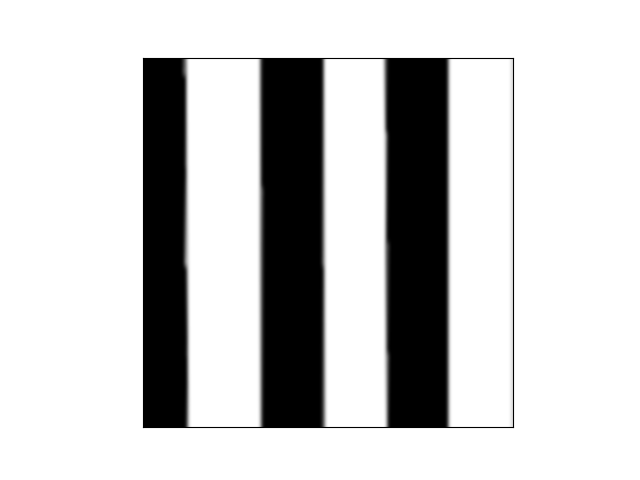
\includegraphics[width=\linewidth]{image/bipolar/97818.png}
      \caption{gamma=0.97818}
    \end{subfigure}%
    \begin{subfigure}{.5\textwidth}
      \centering
      
\includegraphics[width=\linewidth]{image/bipolar/99999.png}
      \caption{gamma=0.99999}
    \end{subfigure}
    \caption{典型情况下的双极系数}
    \end{figure}

\begin{figure}[h]
    \centering
    \begin{subfigure}{.5\textwidth}
        \centering
        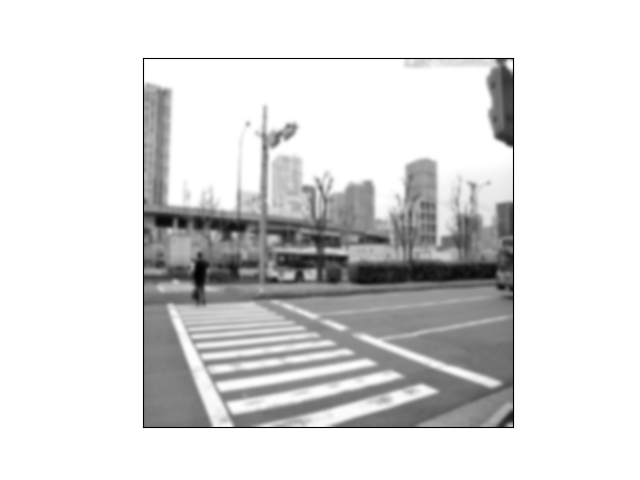
\includegraphics[width=\linewidth]{image/bipolar/64900.png}
        \caption{gamma=0.64900}
    \end{subfigure}%
    \begin{subfigure}{.5\textwidth}
        \centering
        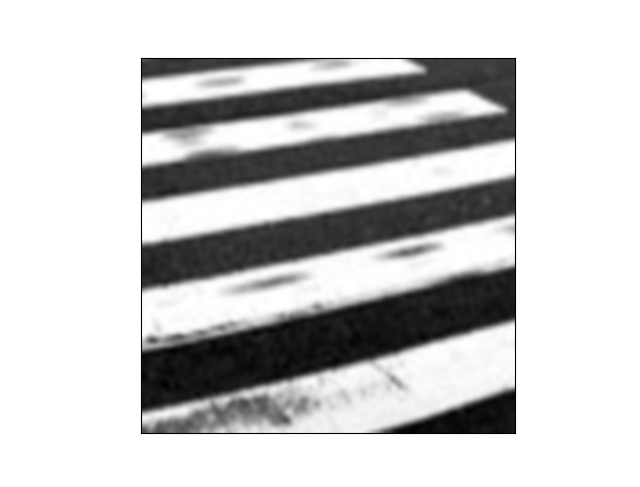
\includegraphics[width=\linewidth]{image/bipolar/72579.png}
        \caption{gamma=0.72579}
    \end{subfigure} \\
    \begin{subfigure}{.5\textwidth}
        \centering
        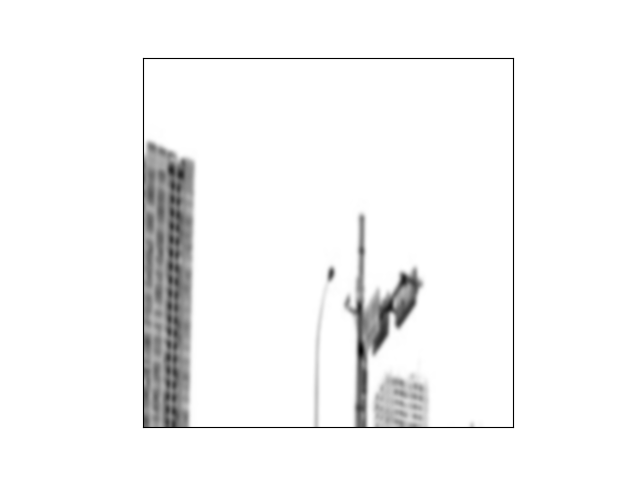
\includegraphics[width=\linewidth]{image/bipolar/29594.png}
        \caption{gamma=0.29594}
    \end{subfigure}%
    \begin{subfigure}{.5\textwidth}
        \centering
        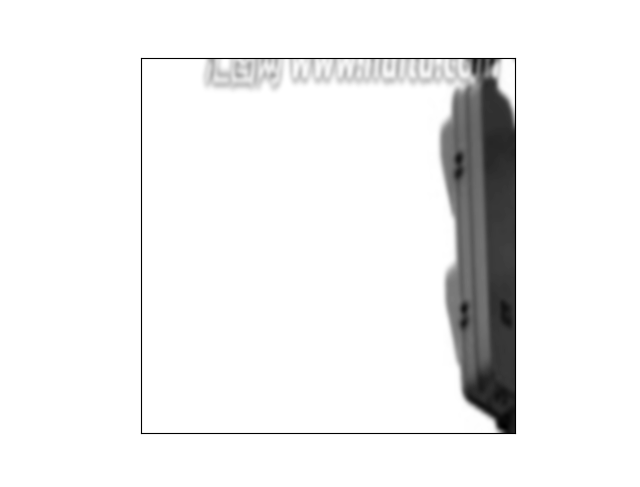
\includegraphics[width=\linewidth]{image/bipolar/90736.png}
        \caption{gamma=0.90736}
    \end{subfigure}
    \caption{现实照片中的双极系数}
    \end{figure}
\par
由以上图像示例说明,对于双极系数的推理是科学的,在现实的照片中也有体现,但仍有误识的情况。可以分析得到,双极系数法在现实情况中确实能反映出斑马线的特征,但方法特异性不高,它主要的门槛在于无法利用图片空间域的信息,比如邻接信息,聚类信息等等,单纯从灰度的统计信息出发难免有局限。
    
\section{Hough变换判据的研究}
我们从空间域特性出发,研究更加细致得斑马线判据。根据斑马线的特性,在ROI中只可能存在一组夹角不大的直线,而且直线之间呈现黑白相间的特点。因此我们可以首先对灰度化的ROI应用边缘检测算子,然后使用直线提取算法。在得到ROI中的一组直线之后,需要做一些特殊处理:
\begin{enumerate}
    \item 首先,要去除法向的干扰直线,做法是通过一个角度为$\frac{\pi}{4}$的滑动扇形来取出夹角在一个扇形以内的最多的直线,然后将其余直线全部删除。原因是即使是考虑如图4-1所示的平视视角也不会出现夹角大于$\frac{\pi}{4}$的斑马线边缘。
    \item 其次,要合并由于边缘检测产生的误差导致的接近重合的直线,如图4-2,在实现当中通过去除像素个数小于1000的区域来实现。
    \item 最后,这一组保留下来的直线,在ROI中不能相交,在实际操作中可以给干扰直线留出一点余量。
\end{enumerate}
\begin{figure}[h]
	\centering
	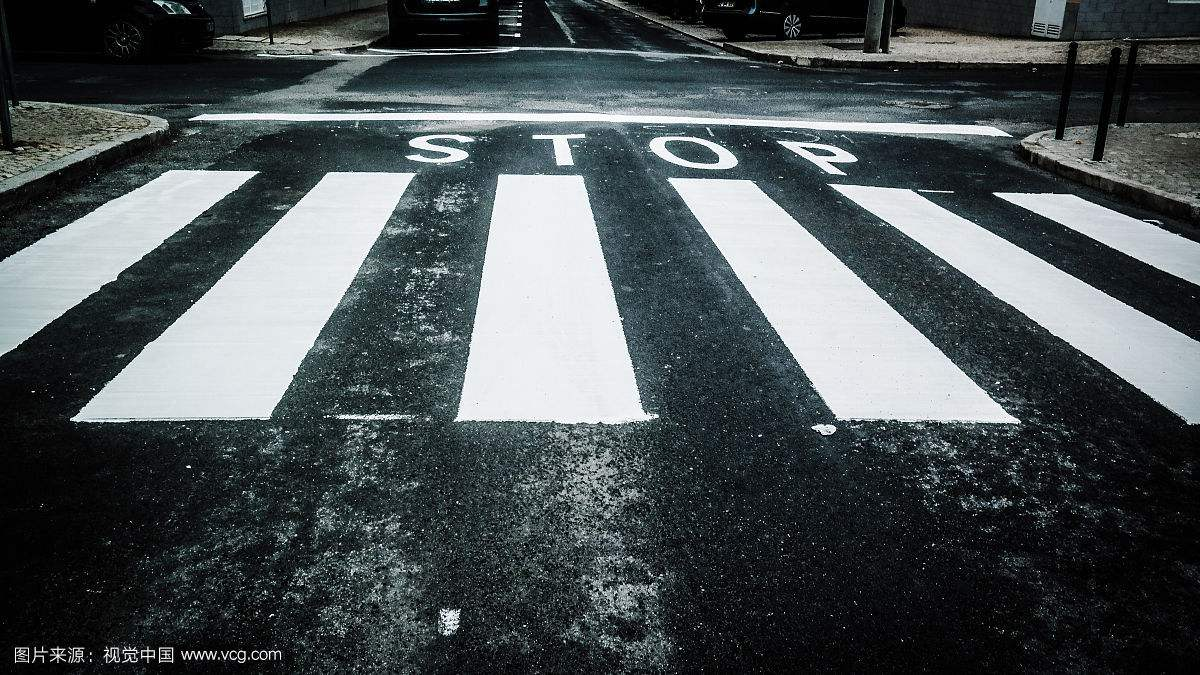
\includegraphics[width=0.5\textwidth]{image/sight.jpeg}
	\caption{平视斑马线}
\end{figure}
\begin{figure}[h]
	\centering
	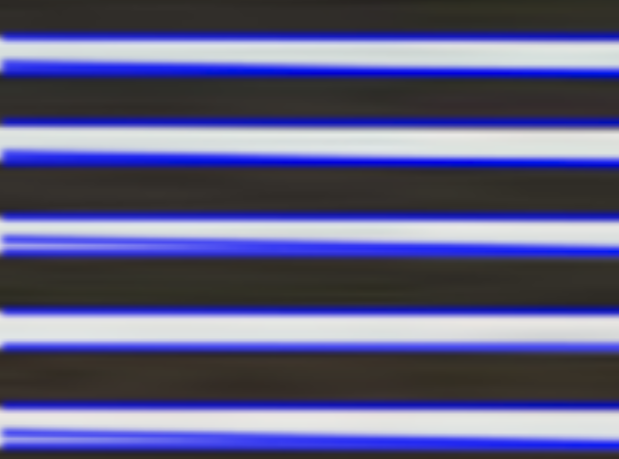
\includegraphics[width=0.5\textwidth]{image/line_merge_cut.png}
    \caption{删除重合直线}
\end{figure}
\par
当我们确定一组方向大致相同且在ROI内不相交的直线之后,我们实际上在二位平面上定义了序关系,我们按照法向遍历这些被直线分割的区域,按照二值化后白色占据绝对优势或者黑色占据绝对优势抑或两者都不是,确定一个形如BWBWBWXBXWBBW的字符串,然后通过字串匹配算法寻找BWBWBW和WBWBWB即可。
\begin{figure}[h]
	\centering
	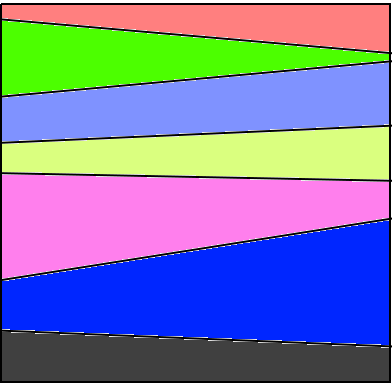
\includegraphics[width=0.5\textwidth]{image/order2.png}
	\caption{平面上的序关系}
\end{figure}

\section{纹理判据与支持向量机}
在实验结果中,Hough变换判据已经取得了不错的识别效果。为了进一步降低误识率提高准确率,我们可以把经过预处理的ROI视为一种纹理,进而使用纹理检测的技术判定斑马线。我们通过计算
\begin{align}
    dist=[1, 3, 5, 9] \\
    angle=[0, \frac{\pi}{4}, \frac{\pi}{2}, \frac{3 \times \pi}{4}, ]
\end{align}
共$16$个灰度共生矩阵,分别提取:熵、对比度、能量、反差分矩、相关性五个特征,构成一个$80$维的特征向量。通过学习算法来检测斑马线纹理。这次实验中我们采用支持向量机作为学习机。纹理判据在测试集上表现为在准确率下降不大的情况下,显著降低了误识率。\par
最终的判定依据为:
\begin{align}
    Predict=\left\{\begin{matrix}
        true & if \frac{\alpha}{4} + \frac{\beta}{4} + \frac{\gamma}{2} \geq \frac{1}{2} \\
        false & otherwise
        \end{matrix}\right.
\end{align}
$\alpha,\beta,\gamma$ 依次为4.1,4.2,4.3中判据的判定结果 